\documentclass[1p]{elsarticle_modified}
%\bibliographystyle{elsarticle-num}

%\usepackage[colorlinks]{hyperref}
%\usepackage{abbrmath_seonhwa} %\Abb, \Ascr, \Acal ,\Abf, \Afrak
\usepackage{amsfonts}
\usepackage{amssymb}
\usepackage{amsmath}
\usepackage{amsthm}
\usepackage{scalefnt}
\usepackage{amsbsy}
\usepackage{kotex}
\usepackage{caption}
\usepackage{subfig}
\usepackage{color}
\usepackage{graphicx}
\usepackage{xcolor} %% white, black, red, green, blue, cyan, magenta, yellow
\usepackage{float}
\usepackage{setspace}
\usepackage{hyperref}

\usepackage{tikz}
\usetikzlibrary{arrows}

\usepackage{multirow}
\usepackage{array} % fixed length table
\usepackage{hhline}

%%%%%%%%%%%%%%%%%%%%%
\makeatletter
\renewcommand*\env@matrix[1][\arraystretch]{%
	\edef\arraystretch{#1}%
	\hskip -\arraycolsep
	\let\@ifnextchar\new@ifnextchar
	\array{*\c@MaxMatrixCols c}}
\makeatother %https://tex.stackexchange.com/questions/14071/how-can-i-increase-the-line-spacing-in-a-matrix
%%%%%%%%%%%%%%%

\usepackage[normalem]{ulem}

\newcommand{\msout}[1]{\ifmmode\text{\sout{\ensuremath{#1}}}\else\sout{#1}\fi}
%SOURCE: \msout is \stkout macro in https://tex.stackexchange.com/questions/20609/strikeout-in-math-mode

\newcommand{\cancel}[1]{
	\ifmmode
	{\color{red}\msout{#1}}
	\else
	{\color{red}\sout{#1}}
	\fi
}

\newcommand{\add}[1]{
	{\color{blue}\uwave{#1}}
}

\newcommand{\replace}[2]{
	\ifmmode
	{\color{red}\msout{#1}}{\color{blue}\uwave{#2}}
	\else
	{\color{red}\sout{#1}}{\color{blue}\uwave{#2}}
	\fi
}

\newcommand{\Sol}{\mathcal{S}} %segment
\newcommand{\D}{D} %diagram
\newcommand{\A}{\mathcal{A}} %arc


%%%%%%%%%%%%%%%%%%%%%%%%%%%%%5 test

\def\sl{\operatorname{\textup{SL}}(2,\Cbb)}
\def\psl{\operatorname{\textup{PSL}}(2,\Cbb)}
\def\quan{\mkern 1mu \triangleright \mkern 1mu}

\theoremstyle{definition}
\newtheorem{thm}{Theorem}[section]
\newtheorem{prop}[thm]{Proposition}
\newtheorem{lem}[thm]{Lemma}
\newtheorem{ques}[thm]{Question}
\newtheorem{cor}[thm]{Corollary}
\newtheorem{defn}[thm]{Definition}
\newtheorem{exam}[thm]{Example}
\newtheorem{rmk}[thm]{Remark}
\newtheorem{alg}[thm]{Algorithm}

\newcommand{\I}{\sqrt{-1}}
\begin{document}

%\begin{frontmatter}
%
%\title{Boundary parabolic representations of knots up to 8 crossings}
%
%%% Group authors per affiliation:
%\author{Yunhi Cho} 
%\address{Department of Mathematics, University of Seoul, Seoul, Korea}
%\ead{yhcho@uos.ac.kr}
%
%
%\author{Seonhwa Kim} %\fnref{s_kim}}
%\address{Center for Geometry and Physics, Institute for Basic Science, Pohang, 37673, Korea}
%\ead{ryeona17@ibs.re.kr}
%
%\author{Hyuk Kim}
%\address{Department of Mathematical Sciences, Seoul National University, Seoul 08826, Korea}
%\ead{hyukkim@snu.ac.kr}
%
%\author{Seokbeom Yoon}
%\address{Department of Mathematical Sciences, Seoul National University, Seoul, 08826,  Korea}
%\ead{sbyoon15@snu.ac.kr}
%
%\begin{abstract}
%We find all boundary parabolic representation of knots up to 8 crossings.
%
%\end{abstract}
%\begin{keyword}
%    \MSC[2010] 57M25 
%\end{keyword}
%
%\end{frontmatter}

%\linenumbers
%\tableofcontents
%
\newcommand\colored[1]{\textcolor{white}{\rule[-0.35ex]{0.8em}{1.4ex}}\kern-0.8em\color{red} #1}%
%\newcommand\colored[1]{\textcolor{white}{ #1}\kern-2.17ex	\textcolor{white}{ #1}\kern-1.81ex	\textcolor{white}{ #1}\kern-2.15ex\color{red}#1	}

{\Large $\underline{12n_{0848}~(K12n_{0848})}$}

\setlength{\tabcolsep}{10pt}
\renewcommand{\arraystretch}{1.6}
\vspace{1cm}\begin{tabular}{m{100pt}>{\centering\arraybackslash}m{274pt}}
\multirow{5}{120pt}{
	\centering
	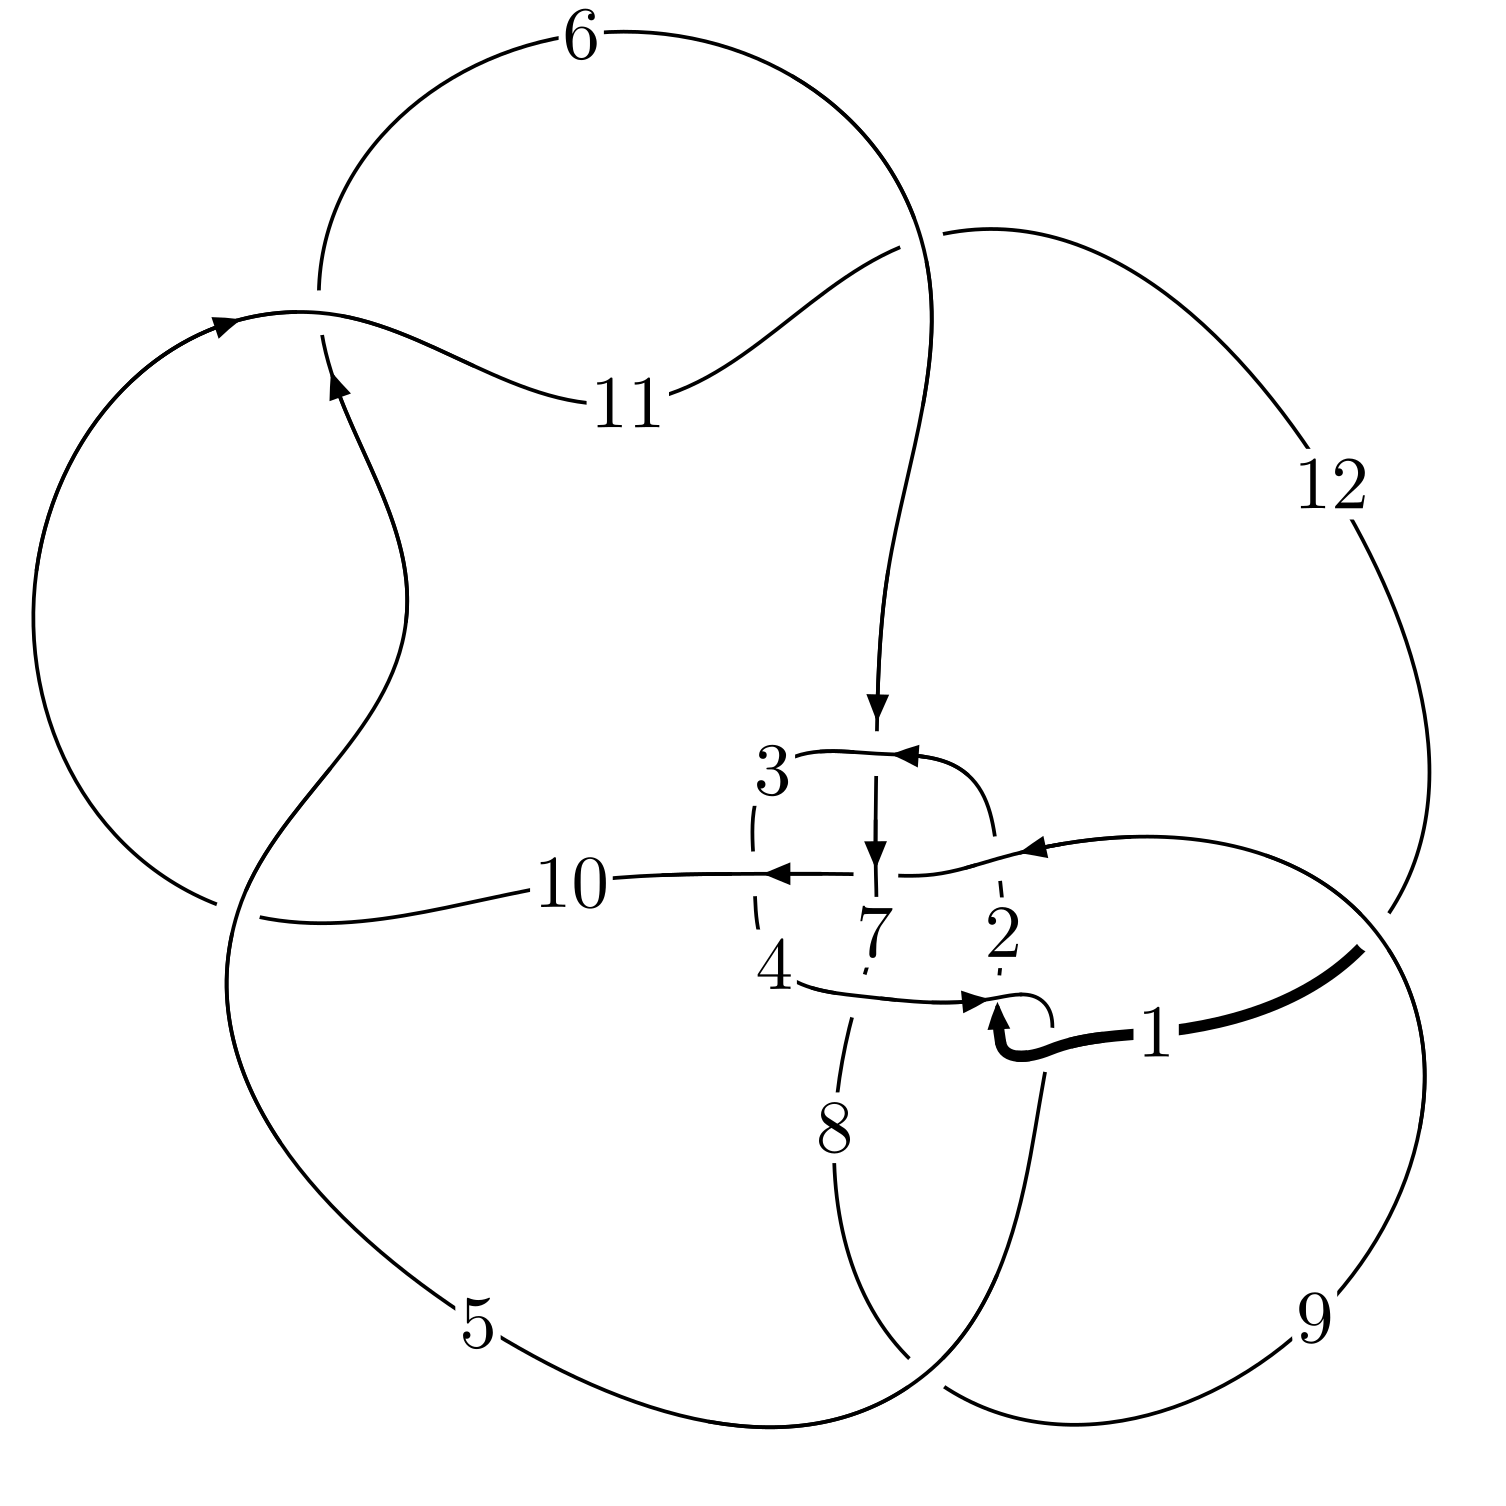
\includegraphics[width=112pt]{../../../GIT/diagram.site/Diagrams/png/2937_12n_0848.png}\\
\ \ \ A knot diagram\footnotemark}&
\allowdisplaybreaks
\textbf{Linearized knot diagam} \\
\cline{2-2}
 &
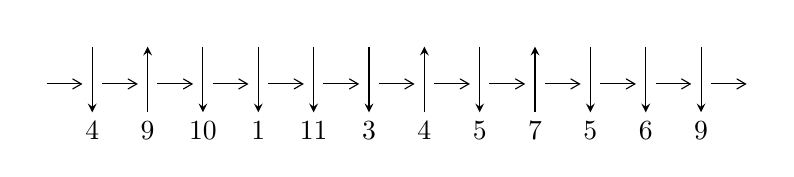
\begin{tikzpicture}[x=20pt, y=17pt]
	% nodes
	\node (C0) at (0, 0) {};
	\node (C1) at (1, 0) {};
	\node (C1U) at (1, +1) {};
	\node (C1D) at (1, -1) {4};

	\node (C2) at (2, 0) {};
	\node (C2U) at (2, +1) {};
	\node (C2D) at (2, -1) {9};

	\node (C3) at (3, 0) {};
	\node (C3U) at (3, +1) {};
	\node (C3D) at (3, -1) {10};

	\node (C4) at (4, 0) {};
	\node (C4U) at (4, +1) {};
	\node (C4D) at (4, -1) {1};

	\node (C5) at (5, 0) {};
	\node (C5U) at (5, +1) {};
	\node (C5D) at (5, -1) {11};

	\node (C6) at (6, 0) {};
	\node (C6U) at (6, +1) {};
	\node (C6D) at (6, -1) {3};

	\node (C7) at (7, 0) {};
	\node (C7U) at (7, +1) {};
	\node (C7D) at (7, -1) {4};

	\node (C8) at (8, 0) {};
	\node (C8U) at (8, +1) {};
	\node (C8D) at (8, -1) {5};

	\node (C9) at (9, 0) {};
	\node (C9U) at (9, +1) {};
	\node (C9D) at (9, -1) {7};

	\node (C10) at (10, 0) {};
	\node (C10U) at (10, +1) {};
	\node (C10D) at (10, -1) {5};

	\node (C11) at (11, 0) {};
	\node (C11U) at (11, +1) {};
	\node (C11D) at (11, -1) {6};

	\node (C12) at (12, 0) {};
	\node (C12U) at (12, +1) {};
	\node (C12D) at (12, -1) {9};
	\node (C13) at (13, 0) {};

	% arrows
	\draw[->,>={angle 60}]
	(C0) edge (C1) (C1) edge (C2) (C2) edge (C3) (C3) edge (C4) (C4) edge (C5) (C5) edge (C6) (C6) edge (C7) (C7) edge (C8) (C8) edge (C9) (C9) edge (C10) (C10) edge (C11) (C11) edge (C12) (C12) edge (C13) ;	\draw[->,>=stealth]
	(C1U) edge (C1D) (C2D) edge (C2U) (C3U) edge (C3D) (C4U) edge (C4D) (C5U) edge (C5D) (C6U) edge (C6D) (C7D) edge (C7U) (C8U) edge (C8D) (C9D) edge (C9U) (C10U) edge (C10D) (C11U) edge (C11D) (C12U) edge (C12D) ;
	\end{tikzpicture} \\
\hhline{~~} \\& 
\textbf{Solving Sequence} \\ \cline{2-2} 
 &
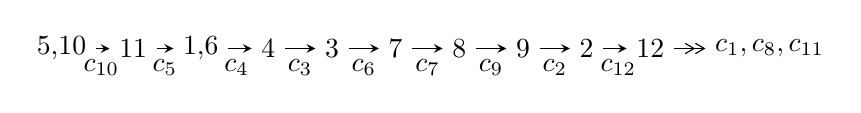
\begin{tikzpicture}[x=23pt, y=7pt]
	% node
	\node (A0) at (-1/8, 0) {5,10};
	\node (A1) at (1, 0) {11};
	\node (A2) at (33/16, 0) {1,6};
	\node (A3) at (25/8, 0) {4};
	\node (A4) at (33/8, 0) {3};
	\node (A5) at (41/8, 0) {7};
	\node (A6) at (49/8, 0) {8};
	\node (A7) at (57/8, 0) {9};
	\node (A8) at (65/8, 0) {2};
	\node (A9) at (73/8, 0) {12};
	\node (C1) at (1/2, -1) {$c_{10}$};
	\node (C2) at (3/2, -1) {$c_{5}$};
	\node (C3) at (21/8, -1) {$c_{4}$};
	\node (C4) at (29/8, -1) {$c_{3}$};
	\node (C5) at (37/8, -1) {$c_{6}$};
	\node (C6) at (45/8, -1) {$c_{7}$};
	\node (C7) at (53/8, -1) {$c_{9}$};
	\node (C8) at (61/8, -1) {$c_{2}$};
	\node (C9) at (69/8, -1) {$c_{12}$};
	\node (A10) at (11, 0) {$c_{1},c_{8},c_{11}$};

	% edge
	\draw[->,>=stealth]	
	(A0) edge (A1) (A1) edge (A2) (A2) edge (A3) (A3) edge (A4) (A4) edge (A5) (A5) edge (A6) (A6) edge (A7) (A7) edge (A8) (A8) edge (A9) ;
	\draw[->>,>={angle 60}]	
	(A9) edge (A10);
\end{tikzpicture} \\ 

\end{tabular} \\

\footnotetext{
The image of knot diagram is generated by the software ``\textbf{Draw programme}" developed by Andrew Bartholomew(\url{http://www.layer8.co.uk/maths/draw/index.htm\#Running-draw}), where we modified some parts for our purpose(\url{https://github.com/CATsTAILs/LinksPainter}).
}\phantom \\ \newline 
\centering \textbf{Ideals for irreducible components\footnotemark of $X_{\text{par}}$} 
 
\begin{align*}
I^u_{1}&=\langle 
1490992711 u^{33}+21038016102 u^{32}+\cdots+104665856 b+191326556928,\\
\phantom{I^u_{1}}&\phantom{= \langle  }746029 u^{33}-897227141 u^{32}+\cdots+313997568 a-74904566272,\;u^{34}+16 u^{33}+\cdots+512 u+256\rangle \\
I^u_{2}&=\langle 
9001 u^{25}-3749 u^{24}+\cdots+24457 b+25814,\;-17555 u^{25}-14121 u^{24}+\cdots+73371 a+84484,\\
\phantom{I^u_{2}}&\phantom{= \langle  }u^{26}-14 u^{24}+\cdots+u+3\rangle \\
I^u_{3}&=\langle 
-6 a^3 b u-4 a^3 b+4 a^2 b u+2 a^2 b- b a u- a^2 u+b^2- b a-2 b u- a^2+2 a u+u-1,\\
\phantom{I^u_{3}}&\phantom{= \langle  }a^4- a^3 u+a^3- a^2 u+2 a^2+2 a u-3 a-3 u+5,\;u^2- u-1\rangle \\
I^u_{4}&=\langle 
-6 a^3 b u-4 a^3 b+8 a^2 b u+4 a^2 b-3 b a u- a^2 u+b^2-3 b a+2 b u- a^2+2 a u+u-1,\\
\phantom{I^u_{4}}&\phantom{= \langle  }a^4-2 a^3 u+2 a^3-2 a^2 u+4 a^2-2 a u+3 a-3 u+5,\;u^2- u-1\rangle \\
I^u_{5}&=\langle 
b- u,\;a,\;u^2+u-1\rangle \\
\\
\end{align*}
\raggedright * 5 irreducible components of $\dim_{\mathbb{C}}=0$, with total 94 representations.\\
\footnotetext{All coefficients of polynomials are rational numbers. But the coefficients are sometimes approximated in decimal forms when there is not enough margin.}
\newpage
\renewcommand{\arraystretch}{1}
\centering \section*{I. $I^u_{1}= \langle 1.49\times10^{9} u^{33}+2.10\times10^{10} u^{32}+\cdots+1.05\times10^{8} b+1.91\times10^{11},\;7.46\times10^{5} u^{33}-8.97\times10^{8} u^{32}+\cdots+3.14\times10^{8} a-7.49\times10^{10},\;u^{34}+16 u^{33}+\cdots+512 u+256 \rangle$}
\flushleft \textbf{(i) Arc colorings}\\
\begin{tabular}{m{7pt} m{180pt} m{7pt} m{180pt} }
\flushright $a_{5}=$&$\begin{pmatrix}0\\u\end{pmatrix}$ \\
\flushright $a_{10}=$&$\begin{pmatrix}1\\0\end{pmatrix}$ \\
\flushright $a_{11}=$&$\begin{pmatrix}1\\u^2\end{pmatrix}$ \\
\flushright $a_{1}=$&$\begin{pmatrix}-0.00237591 u^{33}+2.85743 u^{32}+\cdots+210.618 u+238.551\\-14.2453 u^{33}-201.002 u^{32}+\cdots-2806.15 u-1827.97\end{pmatrix}$ \\
\flushright $a_{6}=$&$\begin{pmatrix}- u\\- u^3+u\end{pmatrix}$ \\
\flushright $a_{4}=$&$\begin{pmatrix}-9.99391 u^{33}-154.470 u^{32}+\cdots-2993.11 u-2567.55\\46.6896 u^{33}+675.692 u^{32}+\cdots+10474.3 u+7478.64\end{pmatrix}$ \\
\flushright $a_{3}=$&$\begin{pmatrix}36.6957 u^{33}+521.222 u^{32}+\cdots+7481.16 u+4911.09\\46.6896 u^{33}+675.692 u^{32}+\cdots+10474.3 u+7478.64\end{pmatrix}$ \\
\flushright $a_{7}=$&$\begin{pmatrix}30.0648 u^{33}+443.715 u^{32}+\cdots+7461.44 u+6086.67\\8.51516 u^{33}+125.472 u^{32}+\cdots+2106.90 u+1857.91\end{pmatrix}$ \\
\flushright $a_{8}=$&$\begin{pmatrix}13.1190 u^{33}+186.388 u^{32}+\cdots+2673.13 u+1806.42\\-28.4932 u^{33}-403.883 u^{32}+\cdots-5742.22 u-3935.80\end{pmatrix}$ \\
\flushright $a_{9}=$&$\begin{pmatrix}-13.1190 u^{33}-186.388 u^{32}+\cdots-2673.13 u-1806.42\\-12.1032 u^{33}-178.316 u^{32}+\cdots-2939.47 u-2084.28\end{pmatrix}$ \\
\flushright $a_{2}=$&$\begin{pmatrix}0.811803 u^{33}+19.0064 u^{32}+\cdots+712.808 u+606.416\\-28.5552 u^{33}-410.268 u^{32}+\cdots-6140.23 u-4213.59\end{pmatrix}$ \\
\flushright $a_{12}=$&$\begin{pmatrix}- u^2+1\\- u^4+2 u^2\end{pmatrix}$\\&\end{tabular}
\flushleft \textbf{(ii) Obstruction class $= -1$}\\~\\
\flushleft \textbf{(iii) Cusp Shapes $= \frac{470816681}{3270808} u^{33}+\frac{27543600709}{13083232} u^{32}+\cdots+\frac{13947213170}{408851} u+\frac{10499734540}{408851}$}\\~\\
\newpage\renewcommand{\arraystretch}{1}
\flushleft \textbf{(iv) u-Polynomials at the component}\newline \\
\begin{tabular}{m{50pt}|m{274pt}}
Crossings & \hspace{64pt}u-Polynomials at each crossing \\
\hline $$\begin{aligned}c_{1},c_{4}\end{aligned}$$&$\begin{aligned}
&u^{34}-9 u^{33}+\cdots-135 u+45
\end{aligned}$\\
\hline $$\begin{aligned}c_{2},c_{7}\end{aligned}$$&$\begin{aligned}
&u^{34}+15 u^{32}+\cdots+3 u+31
\end{aligned}$\\
\hline $$\begin{aligned}c_{3},c_{6}\end{aligned}$$&$\begin{aligned}
&u^{34}+u^{33}+\cdots-2 u+1
\end{aligned}$\\
\hline $$\begin{aligned}c_{5},c_{10},c_{11}\end{aligned}$$&$\begin{aligned}
&u^{34}-16 u^{33}+\cdots-512 u+256
\end{aligned}$\\
\hline $$\begin{aligned}c_{8},c_{12}\end{aligned}$$&$\begin{aligned}
&u^{34}+2 u^{33}+\cdots+2 u+1
\end{aligned}$\\
\hline $$\begin{aligned}c_{9}\end{aligned}$$&$\begin{aligned}
&u^{34}+14 u^{33}+\cdots+540 u+45
\end{aligned}$\\
\hline
\end{tabular}\\~\\
\newpage\renewcommand{\arraystretch}{1}
\flushleft \textbf{(v) Riley Polynomials at the component}\newline \\
\begin{tabular}{m{50pt}|m{274pt}}
Crossings & \hspace{64pt}Riley Polynomials at each crossing \\
\hline $$\begin{aligned}c_{1},c_{4}\end{aligned}$$&$\begin{aligned}
&y^{34}+9 y^{33}+\cdots+7425 y+2025
\end{aligned}$\\
\hline $$\begin{aligned}c_{2},c_{7}\end{aligned}$$&$\begin{aligned}
&y^{34}+30 y^{33}+\cdots+16297 y+961
\end{aligned}$\\
\hline $$\begin{aligned}c_{3},c_{6}\end{aligned}$$&$\begin{aligned}
&y^{34}-25 y^{33}+\cdots-22 y+1
\end{aligned}$\\
\hline $$\begin{aligned}c_{5},c_{10},c_{11}\end{aligned}$$&$\begin{aligned}
&y^{34}-28 y^{33}+\cdots-65536 y+65536
\end{aligned}$\\
\hline $$\begin{aligned}c_{8},c_{12}\end{aligned}$$&$\begin{aligned}
&y^{34}-48 y^{33}+\cdots-10 y+1
\end{aligned}$\\
\hline $$\begin{aligned}c_{9}\end{aligned}$$&$\begin{aligned}
&y^{34}-6 y^{33}+\cdots+31050 y+2025
\end{aligned}$\\
\hline
\end{tabular}\\~\\
\newpage\flushleft \textbf{(vi) Complex Volumes and Cusp Shapes}
$$\begin{array}{c|c|c}  
\text{Solutions to }I^u_{1}& \I (\text{vol} + \sqrt{-1}CS) & \text{Cusp shape}\\
 \hline 
\begin{aligned}
u &= -0.795593 + 0.740595 I \\
a &= -0.290888 + 0.609919 I \\
b &= \phantom{-}0.853986 + 1.101180 I\end{aligned}
 & \phantom{-}3.51064 + 1.64445 I & \phantom{-}7.07709 - 8.00929 I \\ \hline\begin{aligned}
u &= -0.795593 - 0.740595 I \\
a &= -0.290888 - 0.609919 I \\
b &= \phantom{-}0.853986 - 1.101180 I\end{aligned}
 & \phantom{-}3.51064 - 1.64445 I & \phantom{-}7.07709 + 8.00929 I \\ \hline\begin{aligned}
u &= \phantom{-}1.092680 + 0.387055 I \\
a &= -0.383036 - 0.709367 I \\
b &= \phantom{-}1.43819 - 0.26328 I\end{aligned}
 & -0.064466 - 0.761171 I & \phantom{-0.000000 } 0 \\ \hline\begin{aligned}
u &= \phantom{-}1.092680 - 0.387055 I \\
a &= -0.383036 + 0.709367 I \\
b &= \phantom{-}1.43819 + 0.26328 I\end{aligned}
 & -0.064466 + 0.761171 I & \phantom{-0.000000 } 0 \\ \hline\begin{aligned}
u &= \phantom{-}0.697499 + 0.930339 I \\
a &= \phantom{-}0.027330 + 1.123010 I \\
b &= -0.506447 - 0.080887 I\end{aligned}
 & -6.81076 - 4.03336 I & \phantom{-0.000000 } 0 \\ \hline\begin{aligned}
u &= \phantom{-}0.697499 - 0.930339 I \\
a &= \phantom{-}0.027330 - 1.123010 I \\
b &= -0.506447 + 0.080887 I\end{aligned}
 & -6.81076 + 4.03336 I & \phantom{-0.000000 } 0 \\ \hline\begin{aligned}
u &= -0.939424 + 0.738369 I \\
a &= \phantom{-}0.552486 - 0.224603 I \\
b &= -1.85831 - 0.64729 I\end{aligned}
 & \phantom{-}3.08759 + 3.98437 I & \phantom{-0.000000 } 0 \\ \hline\begin{aligned}
u &= -0.939424 - 0.738369 I \\
a &= \phantom{-}0.552486 + 0.224603 I \\
b &= -1.85831 + 0.64729 I\end{aligned}
 & \phantom{-}3.08759 - 3.98437 I & \phantom{-0.000000 } 0 \\ \hline\begin{aligned}
u &= \phantom{-}0.144340 + 0.791374 I \\
a &= \phantom{-}1.60313 - 0.01473 I \\
b &= -1.48435 + 0.51718 I\end{aligned}
 & \phantom{-}2.79908 - 3.47479 I & -8.15502 + 3.50613 I \\ \hline\begin{aligned}
u &= \phantom{-}0.144340 - 0.791374 I \\
a &= \phantom{-}1.60313 + 0.01473 I \\
b &= -1.48435 - 0.51718 I\end{aligned}
 & \phantom{-}2.79908 + 3.47479 I & -8.15502 - 3.50613 I\\
 \hline 
 \end{array}$$\newpage$$\begin{array}{c|c|c}  
\text{Solutions to }I^u_{1}& \I (\text{vol} + \sqrt{-1}CS) & \text{Cusp shape}\\
 \hline 
\begin{aligned}
u &= \phantom{-}0.560287 + 1.062520 I \\
a &= -0.967599 + 0.348568 I \\
b &= \phantom{-}1.58175 - 0.28106 I\end{aligned}
 & -6.28578 - 2.44883 I & \phantom{-0.000000 } 0 \\ \hline\begin{aligned}
u &= \phantom{-}0.560287 - 1.062520 I \\
a &= -0.967599 - 0.348568 I \\
b &= \phantom{-}1.58175 + 0.28106 I\end{aligned}
 & -6.28578 + 2.44883 I & \phantom{-0.000000 } 0 \\ \hline\begin{aligned}
u &= \phantom{-}0.715757 + 1.021220 I \\
a &= -1.114730 + 0.080818 I \\
b &= \phantom{-}1.84474 - 0.41176 I\end{aligned}
 & -5.93132 - 10.98960 I & \phantom{-0.000000 } 0 \\ \hline\begin{aligned}
u &= \phantom{-}0.715757 - 1.021220 I \\
a &= -1.114730 - 0.080818 I \\
b &= \phantom{-}1.84474 + 0.41176 I\end{aligned}
 & -5.93132 + 10.98960 I & \phantom{-0.000000 } 0 \\ \hline\begin{aligned}
u &= \phantom{-}0.664796 + 1.099000 I \\
a &= \phantom{-}0.343002 + 0.963985 I \\
b &= -0.939763 + 0.206515 I\end{aligned}
 & -5.69125 + 4.02411 I & \phantom{-0.000000 } 0 \\ \hline\begin{aligned}
u &= \phantom{-}0.664796 - 1.099000 I \\
a &= \phantom{-}0.343002 - 0.963985 I \\
b &= -0.939763 - 0.206515 I\end{aligned}
 & -5.69125 - 4.02411 I & \phantom{-0.000000 } 0 \\ \hline\begin{aligned}
u &= -1.291770 + 0.282900 I \\
a &= -0.690521 + 0.673761 I \\
b &= \phantom{-}1.16812 + 1.17671 I\end{aligned}
 & -3.78332 + 5.21759 I & \phantom{-0.000000 } 0 \\ \hline\begin{aligned}
u &= -1.291770 - 0.282900 I \\
a &= -0.690521 - 0.673761 I \\
b &= \phantom{-}1.16812 - 1.17671 I\end{aligned}
 & -3.78332 - 5.21759 I & \phantom{-0.000000 } 0 \\ \hline\begin{aligned}
u &= -1.370090 + 0.033595 I \\
a &= -0.889375 + 0.029970 I \\
b &= \phantom{-}0.244301 + 0.277763 I\end{aligned}
 & -6.81111 + 0.91596 I & \phantom{-0.000000 } 0 \\ \hline\begin{aligned}
u &= -1.370090 - 0.033595 I \\
a &= -0.889375 - 0.029970 I \\
b &= \phantom{-}0.244301 - 0.277763 I\end{aligned}
 & -6.81111 - 0.91596 I & \phantom{-0.000000 } 0\\
 \hline 
 \end{array}$$\newpage$$\begin{array}{c|c|c}  
\text{Solutions to }I^u_{1}& \I (\text{vol} + \sqrt{-1}CS) & \text{Cusp shape}\\
 \hline 
\begin{aligned}
u &= -1.351170 + 0.333518 I \\
a &= -0.648443 + 0.927412 I \\
b &= \phantom{-}1.31097 + 1.11405 I\end{aligned}
 & -1.91040 + 7.52741 I & \phantom{-0.000000 } 0 \\ \hline\begin{aligned}
u &= -1.351170 - 0.333518 I \\
a &= -0.648443 - 0.927412 I \\
b &= \phantom{-}1.31097 - 1.11405 I\end{aligned}
 & -1.91040 - 7.52741 I & \phantom{-0.000000 } 0 \\ \hline\begin{aligned}
u &= \phantom{-}0.057196 + 0.549178 I \\
a &= \phantom{-}1.41929 - 0.58161 I \\
b &= -0.916802 + 0.411033 I\end{aligned}
 & \phantom{-}0.35102 - 2.00388 I & -3.74140 + 5.07186 I \\ \hline\begin{aligned}
u &= \phantom{-}0.057196 - 0.549178 I \\
a &= \phantom{-}1.41929 + 0.58161 I \\
b &= -0.916802 - 0.411033 I\end{aligned}
 & \phantom{-}0.35102 + 2.00388 I & -3.74140 - 5.07186 I \\ \hline\begin{aligned}
u &= \phantom{-}0.467415 + 0.199735 I \\
a &= \phantom{-}0.822304 - 0.650309 I \\
b &= \phantom{-}0.404343 + 0.377457 I\end{aligned}
 & -1.146940 - 0.238863 I & -10.78369 + 2.61801 I \\ \hline\begin{aligned}
u &= \phantom{-}0.467415 - 0.199735 I \\
a &= \phantom{-}0.822304 + 0.650309 I \\
b &= \phantom{-}0.404343 - 0.377457 I\end{aligned}
 & -1.146940 + 0.238863 I & -10.78369 - 2.61801 I \\ \hline\begin{aligned}
u &= -1.63628 + 0.32409 I \\
a &= \phantom{-}0.537236 + 0.644759 I \\
b &= -0.368302 - 0.377949 I\end{aligned}
 & -14.4434 + 8.7543 I & \phantom{-0.000000 } 0 \\ \hline\begin{aligned}
u &= -1.63628 - 0.32409 I \\
a &= \phantom{-}0.537236 - 0.644759 I \\
b &= -0.368302 + 0.377949 I\end{aligned}
 & -14.4434 - 8.7543 I & \phantom{-0.000000 } 0 \\ \hline\begin{aligned}
u &= -1.66486 + 0.33880 I \\
a &= \phantom{-}0.668565 - 0.515867 I \\
b &= -2.25117 - 1.06102 I\end{aligned}
 & -13.7374 + 16.0989 I & \phantom{-0.000000 } 0 \\ \hline\begin{aligned}
u &= -1.66486 - 0.33880 I \\
a &= \phantom{-}0.668565 + 0.515867 I \\
b &= -2.25117 + 1.06102 I\end{aligned}
 & -13.7374 - 16.0989 I & \phantom{-0.000000 } 0\\
 \hline 
 \end{array}$$\newpage$$\begin{array}{c|c|c}  
\text{Solutions to }I^u_{1}& \I (\text{vol} + \sqrt{-1}CS) & \text{Cusp shape}\\
 \hline 
\begin{aligned}
u &= -1.66017 + 0.38893 I \\
a &= \phantom{-}0.630339 - 0.408666 I \\
b &= -2.15582 - 1.03899 I\end{aligned}
 & -13.5280 + 7.9597 I & \phantom{-0.000000 } 0 \\ \hline\begin{aligned}
u &= -1.66017 - 0.38893 I \\
a &= \phantom{-}0.630339 + 0.408666 I \\
b &= -2.15582 + 1.03899 I\end{aligned}
 & -13.5280 - 7.9597 I & \phantom{-0.000000 } 0 \\ \hline\begin{aligned}
u &= -1.69061 + 0.34903 I \\
a &= \phantom{-}0.380909 + 0.625669 I \\
b &= -0.365451 + 0.042202 I\end{aligned}
 & -13.49590 + 1.47115 I & \phantom{-0.000000 } 0 \\ \hline\begin{aligned}
u &= -1.69061 - 0.34903 I \\
a &= \phantom{-}0.380909 - 0.625669 I \\
b &= -0.365451 - 0.042202 I\end{aligned}
 & -13.49590 - 1.47115 I & \phantom{-0.000000 } 0\\
 \hline 
 \end{array}$$\newpage\newpage\renewcommand{\arraystretch}{1}
\centering \section*{II. $I^u_{2}= \langle 9001 u^{25}-3749 u^{24}+\cdots+24457 b+25814,\;-17555 u^{25}-14121 u^{24}+\cdots+73371 a+84484,\;u^{26}-14 u^{24}+\cdots+u+3 \rangle$}
\flushleft \textbf{(i) Arc colorings}\\
\begin{tabular}{m{7pt} m{180pt} m{7pt} m{180pt} }
\flushright $a_{5}=$&$\begin{pmatrix}0\\u\end{pmatrix}$ \\
\flushright $a_{10}=$&$\begin{pmatrix}1\\0\end{pmatrix}$ \\
\flushright $a_{11}=$&$\begin{pmatrix}1\\u^2\end{pmatrix}$ \\
\flushright $a_{1}=$&$\begin{pmatrix}0.239263 u^{25}+0.192460 u^{24}+\cdots+0.129438 u-1.15146\\-0.368034 u^{25}+0.153289 u^{24}+\cdots-3.69919 u-1.05549\end{pmatrix}$ \\
\flushright $a_{6}=$&$\begin{pmatrix}- u\\- u^3+u\end{pmatrix}$ \\
\flushright $a_{4}=$&$\begin{pmatrix}0.133486 u^{25}+0.561148 u^{24}+\cdots-2.94220 u+2.26110\\-0.941285 u^{25}+0.413051 u^{24}+\cdots+4.01889 u-0.499203\end{pmatrix}$ \\
\flushright $a_{3}=$&$\begin{pmatrix}-0.807799 u^{25}+0.974200 u^{24}+\cdots+1.07669 u+1.76190\\-0.941285 u^{25}+0.413051 u^{24}+\cdots+4.01889 u-0.499203\end{pmatrix}$ \\
\flushright $a_{7}=$&$\begin{pmatrix}-1.37857 u^{25}+1.35262 u^{24}+\cdots+4.31739 u-4.85565\\-0.395183 u^{25}-0.0794864 u^{24}+\cdots+0.306006 u+0.0778509\end{pmatrix}$ \\
\flushright $a_{8}=$&$\begin{pmatrix}0.386869 u^{25}+0.659811 u^{24}+\cdots-5.29940 u-0.572161\\-0.474670 u^{25}-1.13448 u^{24}+\cdots-0.220959 u+0.263401\end{pmatrix}$ \\
\flushright $a_{9}=$&$\begin{pmatrix}0.386869 u^{25}+0.659811 u^{24}+\cdots-5.29940 u-0.572161\\-0.319091 u^{25}-0.428589 u^{24}+\cdots-2.04138 u-1.71603\end{pmatrix}$ \\
\flushright $a_{2}=$&$\begin{pmatrix}-0.217225 u^{25}+1.32330 u^{24}+\cdots-5.90926 u+3.22244\\-1.02441 u^{25}+1.62354 u^{24}+\cdots-1.93961 u-5.52018\end{pmatrix}$ \\
\flushright $a_{12}=$&$\begin{pmatrix}- u^2+1\\- u^4+2 u^2\end{pmatrix}$\\&\end{tabular}
\flushleft \textbf{(ii) Obstruction class $= 1$}\\~\\
\flushleft \textbf{(iii) Cusp Shapes $= \frac{49040}{24457} u^{25}+\frac{47416}{24457} u^{24}+\cdots+\frac{432909}{24457} u-\frac{279738}{24457}$}\\~\\
\newpage\renewcommand{\arraystretch}{1}
\flushleft \textbf{(iv) u-Polynomials at the component}\newline \\
\begin{tabular}{m{50pt}|m{274pt}}
Crossings & \hspace{64pt}u-Polynomials at each crossing \\
\hline $$\begin{aligned}c_{1}\end{aligned}$$&$\begin{aligned}
&u^{26}-10 u^{25}+\cdots-7 u+1
\end{aligned}$\\
\hline $$\begin{aligned}c_{2},c_{7}\end{aligned}$$&$\begin{aligned}
&u^{26}+u^{25}+\cdots+u+1
\end{aligned}$\\
\hline $$\begin{aligned}c_{3},c_{6}\end{aligned}$$&$\begin{aligned}
&u^{26}+3 u^{24}+\cdots+2 u+1
\end{aligned}$\\
\hline $$\begin{aligned}c_{4}\end{aligned}$$&$\begin{aligned}
&u^{26}+10 u^{25}+\cdots+7 u+1
\end{aligned}$\\
\hline $$\begin{aligned}c_{5}\end{aligned}$$&$\begin{aligned}
&u^{26}-14 u^{24}+\cdots- u+3
\end{aligned}$\\
\hline $$\begin{aligned}c_{8},c_{12}\end{aligned}$$&$\begin{aligned}
&u^{26}- u^{25}+\cdots-2 u+1
\end{aligned}$\\
\hline $$\begin{aligned}c_{9}\end{aligned}$$&$\begin{aligned}
&u^{26}-15 u^{25}+\cdots-3 u^2+1
\end{aligned}$\\
\hline $$\begin{aligned}c_{10},c_{11}\end{aligned}$$&$\begin{aligned}
&u^{26}-14 u^{24}+\cdots+u+3
\end{aligned}$\\
\hline
\end{tabular}\\~\\
\newpage\renewcommand{\arraystretch}{1}
\flushleft \textbf{(v) Riley Polynomials at the component}\newline \\
\begin{tabular}{m{50pt}|m{274pt}}
Crossings & \hspace{64pt}Riley Polynomials at each crossing \\
\hline $$\begin{aligned}c_{1},c_{4}\end{aligned}$$&$\begin{aligned}
&y^{26}+8 y^{25}+\cdots+25 y+1
\end{aligned}$\\
\hline $$\begin{aligned}c_{2},c_{7}\end{aligned}$$&$\begin{aligned}
&y^{26}+9 y^{25}+\cdots+y+1
\end{aligned}$\\
\hline $$\begin{aligned}c_{3},c_{6}\end{aligned}$$&$\begin{aligned}
&y^{26}+6 y^{25}+\cdots-2 y+1
\end{aligned}$\\
\hline $$\begin{aligned}c_{5},c_{10},c_{11}\end{aligned}$$&$\begin{aligned}
&y^{26}-28 y^{25}+\cdots-139 y+9
\end{aligned}$\\
\hline $$\begin{aligned}c_{8},c_{12}\end{aligned}$$&$\begin{aligned}
&y^{26}- y^{25}+\cdots+10 y+1
\end{aligned}$\\
\hline $$\begin{aligned}c_{9}\end{aligned}$$&$\begin{aligned}
&y^{26}-7 y^{25}+\cdots-6 y+1
\end{aligned}$\\
\hline
\end{tabular}\\~\\
\newpage\flushleft \textbf{(vi) Complex Volumes and Cusp Shapes}
$$\begin{array}{c|c|c}  
\text{Solutions to }I^u_{2}& \I (\text{vol} + \sqrt{-1}CS) & \text{Cusp shape}\\
 \hline 
\begin{aligned}
u &= \phantom{-}0.893260 + 0.637608 I \\
a &= \phantom{-}0.560326 + 0.364777 I \\
b &= -2.06321 + 0.72664 I\end{aligned}
 & \phantom{-}3.35683 - 4.09621 I & \phantom{-}9.04442 + 9.36453 I \\ \hline\begin{aligned}
u &= \phantom{-}0.893260 - 0.637608 I \\
a &= \phantom{-}0.560326 - 0.364777 I \\
b &= -2.06321 - 0.72664 I\end{aligned}
 & \phantom{-}3.35683 + 4.09621 I & \phantom{-}9.04442 - 9.36453 I \\ \hline\begin{aligned}
u &= \phantom{-}0.880673 + 0.813599 I \\
a &= -0.199661 - 0.634313 I \\
b &= \phantom{-}0.933273 - 0.889664 I\end{aligned}
 & \phantom{-}3.23266 - 1.47692 I & -14.8020 - 4.6669 I \\ \hline\begin{aligned}
u &= \phantom{-}0.880673 - 0.813599 I \\
a &= -0.199661 + 0.634313 I \\
b &= \phantom{-}0.933273 + 0.889664 I\end{aligned}
 & \phantom{-}3.23266 + 1.47692 I & -14.8020 + 4.6669 I \\ \hline\begin{aligned}
u &= -1.185480 + 0.207955 I \\
a &= -0.955887 + 0.901453 I \\
b &= \phantom{-}0.811448 + 0.957313 I\end{aligned}
 & -4.63801 + 5.99993 I & -14.9211 - 9.9188 I \\ \hline\begin{aligned}
u &= -1.185480 - 0.207955 I \\
a &= -0.955887 - 0.901453 I \\
b &= \phantom{-}0.811448 - 0.957313 I\end{aligned}
 & -4.63801 - 5.99993 I & -14.9211 + 9.9188 I \\ \hline\begin{aligned}
u &= \phantom{-}1.202230 + 0.117764 I \\
a &= -0.637447 - 0.487886 I \\
b &= \phantom{-}2.06384 - 0.07791 I\end{aligned}
 & -0.49786 - 5.55128 I & -9.12515 + 7.27164 I \\ \hline\begin{aligned}
u &= \phantom{-}1.202230 - 0.117764 I \\
a &= -0.637447 + 0.487886 I \\
b &= \phantom{-}2.06384 + 0.07791 I\end{aligned}
 & -0.49786 + 5.55128 I & -9.12515 - 7.27164 I \\ \hline\begin{aligned}
u &= \phantom{-}1.243290 + 0.193806 I \\
a &= -0.489545 - 0.716730 I \\
b &= \phantom{-}1.52007 + 0.02768 I\end{aligned}
 & \phantom{-}0.692396 + 0.908891 I & -7.23329 - 0.60855 I \\ \hline\begin{aligned}
u &= \phantom{-}1.243290 - 0.193806 I \\
a &= -0.489545 + 0.716730 I \\
b &= \phantom{-}1.52007 - 0.02768 I\end{aligned}
 & \phantom{-}0.692396 - 0.908891 I & -7.23329 + 0.60855 I\\
 \hline 
 \end{array}$$\newpage$$\begin{array}{c|c|c}  
\text{Solutions to }I^u_{2}& \I (\text{vol} + \sqrt{-1}CS) & \text{Cusp shape}\\
 \hline 
\begin{aligned}
u &= -0.658052 + 0.322237 I \\
a &= -0.42930 - 1.84882 I \\
b &= \phantom{-}0.1212750 - 0.0229366 I\end{aligned}
 & -2.72945 - 3.92062 I & -4.89712 + 0.84761 I \\ \hline\begin{aligned}
u &= -0.658052 - 0.322237 I \\
a &= -0.42930 + 1.84882 I \\
b &= \phantom{-}0.1212750 + 0.0229366 I\end{aligned}
 & -2.72945 + 3.92062 I & -4.89712 - 0.84761 I \\ \hline\begin{aligned}
u &= \phantom{-}0.253711 + 0.648614 I \\
a &= \phantom{-}1.54093 + 0.37558 I \\
b &= -1.54024 + 0.65815 I\end{aligned}
 & \phantom{-}3.74733 - 3.59988 I & \phantom{-}2.14910 + 5.61503 I \\ \hline\begin{aligned}
u &= \phantom{-}0.253711 - 0.648614 I \\
a &= \phantom{-}1.54093 - 0.37558 I \\
b &= -1.54024 - 0.65815 I\end{aligned}
 & \phantom{-}3.74733 + 3.59988 I & \phantom{-}2.14910 - 5.61503 I \\ \hline\begin{aligned}
u &= -1.323060 + 0.064355 I \\
a &= -0.913064 - 0.390548 I \\
b &= \phantom{-}0.186999 - 0.379225 I\end{aligned}
 & -6.94880 - 1.74984 I & -16.2080 + 5.2909 I \\ \hline\begin{aligned}
u &= -1.323060 - 0.064355 I \\
a &= -0.913064 + 0.390548 I \\
b &= \phantom{-}0.186999 + 0.379225 I\end{aligned}
 & -6.94880 + 1.74984 I & -16.2080 - 5.2909 I \\ \hline\begin{aligned}
u &= \phantom{-}0.523416 + 0.235808 I \\
a &= -0.028987 + 1.090670 I \\
b &= -1.72849 + 0.71878 I\end{aligned}
 & \phantom{-}1.85328 + 4.23193 I & \phantom{-}1.90603 - 3.22437 I \\ \hline\begin{aligned}
u &= \phantom{-}0.523416 - 0.235808 I \\
a &= -0.028987 - 1.090670 I \\
b &= -1.72849 - 0.71878 I\end{aligned}
 & \phantom{-}1.85328 - 4.23193 I & \phantom{-}1.90603 + 3.22437 I \\ \hline\begin{aligned}
u &= -1.39226 + 0.31614 I \\
a &= -0.575637 + 0.854749 I \\
b &= \phantom{-}1.37916 + 1.22716 I\end{aligned}
 & -1.47076 + 7.28765 I & -1.27616 - 2.61256 I \\ \hline\begin{aligned}
u &= -1.39226 - 0.31614 I \\
a &= -0.575637 - 0.854749 I \\
b &= \phantom{-}1.37916 - 1.22716 I\end{aligned}
 & -1.47076 - 7.28765 I & -1.27616 + 2.61256 I\\
 \hline 
 \end{array}$$\newpage$$\begin{array}{c|c|c}  
\text{Solutions to }I^u_{2}& \I (\text{vol} + \sqrt{-1}CS) & \text{Cusp shape}\\
 \hline 
\begin{aligned}
u &= -0.424309 + 0.245639 I \\
a &= -2.57995 + 0.40653 I \\
b &= \phantom{-}0.973329 - 0.091897 I\end{aligned}
 & -3.57929 + 2.94101 I & -6.02456 - 4.67234 I \\ \hline\begin{aligned}
u &= -0.424309 - 0.245639 I \\
a &= -2.57995 - 0.40653 I \\
b &= \phantom{-}0.973329 + 0.091897 I\end{aligned}
 & -3.57929 - 2.94101 I & -6.02456 + 4.67234 I \\ \hline\begin{aligned}
u &= \phantom{-}1.62079 + 0.00745 I \\
a &= \phantom{-}0.614461 + 0.601198 I \\
b &= -1.63692 + 0.02907 I\end{aligned}
 & -11.33640 - 3.61266 I & -11.52145 + 2.34970 I \\ \hline\begin{aligned}
u &= \phantom{-}1.62079 - 0.00745 I \\
a &= \phantom{-}0.614461 - 0.601198 I \\
b &= -1.63692 - 0.02907 I\end{aligned}
 & -11.33640 + 3.61266 I & -11.52145 - 2.34970 I \\ \hline\begin{aligned}
u &= -1.63421 + 0.00977 I \\
a &= -0.072905 - 0.173246 I \\
b &= \phantom{-}1.47945 - 0.36272 I\end{aligned}
 & -6.35593 + 3.58442 I & -8.09065 - 3.04488 I \\ \hline\begin{aligned}
u &= -1.63421 - 0.00977 I \\
a &= -0.072905 + 0.173246 I \\
b &= \phantom{-}1.47945 + 0.36272 I\end{aligned}
 & -6.35593 - 3.58442 I & -8.09065 + 3.04488 I\\
 \hline 
 \end{array}$$\newpage\newpage\renewcommand{\arraystretch}{1}
\centering \section*{III. $I^u_{3}= \langle -6 a^3 b u+4 a^2 b u+\cdots- a^2-1,\;- a^3 u- a^2 u+\cdots-3 a+5,\;u^2- u-1 \rangle$}
\flushleft \textbf{(i) Arc colorings}\\
\begin{tabular}{m{7pt} m{180pt} m{7pt} m{180pt} }
\flushright $a_{5}=$&$\begin{pmatrix}0\\u\end{pmatrix}$ \\
\flushright $a_{10}=$&$\begin{pmatrix}1\\0\end{pmatrix}$ \\
\flushright $a_{11}=$&$\begin{pmatrix}1\\u+1\end{pmatrix}$ \\
\flushright $a_{1}=$&$\begin{pmatrix}a\\b\end{pmatrix}$ \\
\flushright $a_{6}=$&$\begin{pmatrix}- u\\- u-1\end{pmatrix}$ \\
\flushright $a_{4}=$&$\begin{pmatrix}a^2 u\\b a u+u\end{pmatrix}$ \\
\flushright $a_{3}=$&$\begin{pmatrix}b a u+a^2 u+u\\b a u+u\end{pmatrix}$ \\
\flushright $a_{7}=$&$\begin{pmatrix}a^3 b u+a^3 b+a^2 u+a^2-2 a u-1\\-2 a^3 u- a^3+a^2 u+a^2- a u-1\end{pmatrix}$ \\
\flushright $a_{8}=$&$\begin{pmatrix}- a^2 b u-2 a^3 u- a^3+a^2 u+a^2-2 a u\\2 a^2 b u+3 a^3 u+a^2 b+2 a^3- a^2 u+2 a u+2 a\end{pmatrix}$ \\
\flushright $a_{9}=$&$\begin{pmatrix}a^2 b u+2 a^3 u+a^3- a^2 u- a^2+2 a u\\2 a^3 u+a^3-2 a^2 u-2 a^2+2 a u\end{pmatrix}$ \\
\flushright $a_{2}=$&$\begin{pmatrix}a^3 u+a^3+a\\a^2 b u+a^2 b+a u+b+a\end{pmatrix}$ \\
\flushright $a_{12}=$&$\begin{pmatrix}- u\\- u\end{pmatrix}$\\&\end{tabular}
\flushleft \textbf{(ii) Obstruction class $= -1$}\\~\\
\flushleft \textbf{(iii) Cusp Shapes $= -8 a^3 u-4 a^3+12 a^2 u+12 a^2-8 a u-10$}\\~\\
\newpage\renewcommand{\arraystretch}{1}
\flushleft \textbf{(iv) u-Polynomials at the component}\newline \\
\begin{tabular}{m{50pt}|m{274pt}}
Crossings & \hspace{64pt}u-Polynomials at each crossing \\
\hline $$\begin{aligned}c_{1},c_{4}\end{aligned}$$&$\begin{aligned}
&(u^4+u^3+u^2- u+1)^4
\end{aligned}$\\
\hline $$\begin{aligned}c_{2},c_{7}\end{aligned}$$&$\begin{aligned}
&u^{16}+2 u^{15}+\cdots+138 u+379
\end{aligned}$\\
\hline $$\begin{aligned}c_{3},c_{6}\end{aligned}$$&$\begin{aligned}
&u^{16}+u^{15}+\cdots+56 u+59
\end{aligned}$\\
\hline $$\begin{aligned}c_{5},c_{10},c_{11}\end{aligned}$$&$\begin{aligned}
&(u^2+u-1)^8
\end{aligned}$\\
\hline $$\begin{aligned}c_{8},c_{12}\end{aligned}$$&$\begin{aligned}
&u^{16}- u^{15}+\cdots+284 u+59
\end{aligned}$\\
\hline $$\begin{aligned}c_{9}\end{aligned}$$&$\begin{aligned}
&(u^4- u^3+u^2+u+1)^4
\end{aligned}$\\
\hline
\end{tabular}\\~\\
\newpage\renewcommand{\arraystretch}{1}
\flushleft \textbf{(v) Riley Polynomials at the component}\newline \\
\begin{tabular}{m{50pt}|m{274pt}}
Crossings & \hspace{64pt}Riley Polynomials at each crossing \\
\hline $$\begin{aligned}c_{1},c_{4},c_{9}\end{aligned}$$&$\begin{aligned}
&(y^4+y^3+5 y^2+y+1)^4
\end{aligned}$\\
\hline $$\begin{aligned}c_{2},c_{7}\end{aligned}$$&$\begin{aligned}
&y^{16}+16 y^{15}+\cdots+431966 y+143641
\end{aligned}$\\
\hline $$\begin{aligned}c_{3},c_{6}\end{aligned}$$&$\begin{aligned}
&y^{16}+7 y^{15}+\cdots-9862 y+3481
\end{aligned}$\\
\hline $$\begin{aligned}c_{5},c_{10},c_{11}\end{aligned}$$&$\begin{aligned}
&(y^2-3 y+1)^8
\end{aligned}$\\
\hline $$\begin{aligned}c_{8},c_{12}\end{aligned}$$&$\begin{aligned}
&y^{16}- y^{15}+\cdots-39710 y+3481
\end{aligned}$\\
\hline
\end{tabular}\\~\\
\newpage\flushleft \textbf{(vi) Complex Volumes and Cusp Shapes}
$$\begin{array}{c|c|c}  
\text{Solutions to }I^u_{3}& \I (\text{vol} + \sqrt{-1}CS) & \text{Cusp shape}\\
 \hline 
\begin{aligned}
u &= -0.618034\phantom{ +0.000000I} \\
a &= \phantom{-}0.701224 + 0.850806 I \\
b &= \phantom{-}0.921506 + 0.765153 I\end{aligned}
 & \phantom{-}1.25412 - 4.68603 I & -8.70941 + 10.27938 I \\ \hline\begin{aligned}
u &= -0.618034\phantom{ +0.000000I} \\
a &= \phantom{-}0.701224 + 0.850806 I \\
b &= -2.34307 + 0.30970 I\end{aligned}
 & \phantom{-}1.25412 - 4.68603 I & -8.70941 + 10.27938 I \\ \hline\begin{aligned}
u &= -0.618034\phantom{ +0.000000I} \\
a &= \phantom{-}0.701224 - 0.850806 I \\
b &= \phantom{-}0.921506 - 0.765153 I\end{aligned}
 & \phantom{-}1.25412 + 4.68603 I & -8.70941 - 10.27938 I \\ \hline\begin{aligned}
u &= -0.618034\phantom{ +0.000000I} \\
a &= \phantom{-}0.701224 - 0.850806 I \\
b &= -2.34307 - 0.30970 I\end{aligned}
 & \phantom{-}1.25412 + 4.68603 I & -8.70941 - 10.27938 I \\ \hline\begin{aligned}
u &= -0.618034\phantom{ +0.000000I} \\
a &= -1.51024 + 1.83240 I \\
b &= \phantom{-}0.658617 + 0.576443 I\end{aligned}
 & -3.22804 + 4.68603 I & -11.2906 - 10.2794 I \\ \hline\begin{aligned}
u &= -0.618034\phantom{ +0.000000I} \\
a &= -1.51024 + 1.83240 I \\
b &= \phantom{-}0.453931 - 0.626400 I\end{aligned}
 & -3.22804 + 4.68603 I & -11.2906 - 10.2794 I \\ \hline\begin{aligned}
u &= -0.618034\phantom{ +0.000000I} \\
a &= -1.51024 - 1.83240 I \\
b &= \phantom{-}0.658617 - 0.576443 I\end{aligned}
 & -3.22804 - 4.68603 I & -11.2906 + 10.2794 I \\ \hline\begin{aligned}
u &= -0.618034\phantom{ +0.000000I} \\
a &= -1.51024 - 1.83240 I \\
b &= \phantom{-}0.453931 + 0.626400 I\end{aligned}
 & -3.22804 - 4.68603 I & -11.2906 + 10.2794 I \\ \hline\begin{aligned}
u &= \phantom{-}1.61803\phantom{ +0.000000I} \\
a &= \phantom{-}0.576861 + 0.699914 I \\
b &= -1.43394 + 0.81776 I\end{aligned}
 & -11.12370 - 4.68603 I & -11.2906 + 10.2794 I \\ \hline\begin{aligned}
u &= \phantom{-}1.61803\phantom{ +0.000000I} \\
a &= \phantom{-}0.576861 + 0.699914 I \\
b &= -1.47875 - 0.94855 I\end{aligned}
 & -11.12370 - 4.68603 I & -11.2906 + 10.2794 I\\
 \hline 
 \end{array}$$\newpage$$\begin{array}{c|c|c}  
\text{Solutions to }I^u_{3}& \I (\text{vol} + \sqrt{-1}CS) & \text{Cusp shape}\\
 \hline 
\begin{aligned}
u &= \phantom{-}1.61803\phantom{ +0.000000I} \\
a &= \phantom{-}0.576861 - 0.699914 I \\
b &= -1.43394 - 0.81776 I\end{aligned}
 & -11.12370 + 4.68603 I & -11.2906 - 10.2794 I \\ \hline\begin{aligned}
u &= \phantom{-}1.61803\phantom{ +0.000000I} \\
a &= \phantom{-}0.576861 - 0.699914 I \\
b &= -1.47875 + 0.94855 I\end{aligned}
 & -11.12370 + 4.68603 I & -11.2906 - 10.2794 I \\ \hline\begin{aligned}
u &= \phantom{-}1.61803\phantom{ +0.000000I} \\
a &= -0.267844 + 0.324979 I \\
b &= \phantom{-}0.169969 + 0.304317 I\end{aligned}
 & -6.64156 + 4.68603 I & -8.70941 - 10.27938 I \\ \hline\begin{aligned}
u &= \phantom{-}1.61803\phantom{ +0.000000I} \\
a &= -0.267844 + 0.324979 I \\
b &= \phantom{-}3.55174 + 2.50968 I\end{aligned}
 & -6.64156 + 4.68603 I & -8.70941 - 10.27938 I \\ \hline\begin{aligned}
u &= \phantom{-}1.61803\phantom{ +0.000000I} \\
a &= -0.267844 - 0.324979 I \\
b &= \phantom{-}0.169969 - 0.304317 I\end{aligned}
 & -6.64156 - 4.68603 I & -8.70941 + 10.27938 I \\ \hline\begin{aligned}
u &= \phantom{-}1.61803\phantom{ +0.000000I} \\
a &= -0.267844 - 0.324979 I \\
b &= \phantom{-}3.55174 - 2.50968 I\end{aligned}
 & -6.64156 - 4.68603 I & -8.70941 + 10.27938 I\\
 \hline 
 \end{array}$$\newpage\newpage\renewcommand{\arraystretch}{1}
\centering \section*{IV. $I^u_{4}= \langle -6 a^3 b u+8 a^2 b u+\cdots- a^2-1,\;-2 a^3 u-2 a^2 u+\cdots+3 a+5,\;u^2- u-1 \rangle$}
\flushleft \textbf{(i) Arc colorings}\\
\begin{tabular}{m{7pt} m{180pt} m{7pt} m{180pt} }
\flushright $a_{5}=$&$\begin{pmatrix}0\\u\end{pmatrix}$ \\
\flushright $a_{10}=$&$\begin{pmatrix}1\\0\end{pmatrix}$ \\
\flushright $a_{11}=$&$\begin{pmatrix}1\\u+1\end{pmatrix}$ \\
\flushright $a_{1}=$&$\begin{pmatrix}a\\b\end{pmatrix}$ \\
\flushright $a_{6}=$&$\begin{pmatrix}- u\\- u-1\end{pmatrix}$ \\
\flushright $a_{4}=$&$\begin{pmatrix}a^2 u\\b a u+u\end{pmatrix}$ \\
\flushright $a_{3}=$&$\begin{pmatrix}b a u+a^2 u+u\\b a u+u\end{pmatrix}$ \\
\flushright $a_{7}=$&$\begin{pmatrix}a^3 b u+a^3 b+4 a^3 u+2 a^3- a^2 u- a^2+2 a u-1\\a u-1\end{pmatrix}$ \\
\flushright $a_{8}=$&$\begin{pmatrix}- a^3 b u- a^3 b+2 a^2 b u-2 a^3 u- a^3+a^2 u- b a+b u+a^2+a u- b\\3 a^3 b u-4 a^2 b u+\cdots- a-1\end{pmatrix}$ \\
\flushright $a_{9}=$&$\begin{pmatrix}a^3 b u+a^3 b-2 a^2 b u+2 a^3 u+a^3- a^2 u+b a- b u- a^2- a u+b\\a^2 u+a^2-2 a u+1\end{pmatrix}$ \\
\flushright $a_{2}=$&$\begin{pmatrix}a^3 u+a^3+a\\a^2 b u+a^2 b+a u+b+a\end{pmatrix}$ \\
\flushright $a_{12}=$&$\begin{pmatrix}- u\\- u\end{pmatrix}$\\&\end{tabular}
\flushleft \textbf{(ii) Obstruction class $= -1$}\\~\\
\flushleft \textbf{(iii) Cusp Shapes $= 16 a^3 u+8 a^3-12 a^2 u-12 a^2+4 a u-10$}\\~\\
\newpage\renewcommand{\arraystretch}{1}
\flushleft \textbf{(iv) u-Polynomials at the component}\newline \\
\begin{tabular}{m{50pt}|m{274pt}}
Crossings & \hspace{64pt}u-Polynomials at each crossing \\
\hline $$\begin{aligned}c_{1},c_{4}\end{aligned}$$&$\begin{aligned}
&(u^4+2 u^3+2 u^2+u+1)^4
\end{aligned}$\\
\hline $$\begin{aligned}c_{2},c_{7}\end{aligned}$$&$\begin{aligned}
&u^{16}- u^{15}+\cdots+140 u+31
\end{aligned}$\\
\hline $$\begin{aligned}c_{3},c_{6}\end{aligned}$$&$\begin{aligned}
&u^{16}-2 u^{14}+\cdots-50 u+19
\end{aligned}$\\
\hline $$\begin{aligned}c_{5},c_{10},c_{11}\end{aligned}$$&$\begin{aligned}
&(u^2+u-1)^8
\end{aligned}$\\
\hline $$\begin{aligned}c_{8},c_{12}\end{aligned}$$&$\begin{aligned}
&u^{16}-10 u^{14}+\cdots-348 u+181
\end{aligned}$\\
\hline $$\begin{aligned}c_{9}\end{aligned}$$&$\begin{aligned}
&(u^4-2 u^3+2 u^2- u+1)^4
\end{aligned}$\\
\hline
\end{tabular}\\~\\
\newpage\renewcommand{\arraystretch}{1}
\flushleft \textbf{(v) Riley Polynomials at the component}\newline \\
\begin{tabular}{m{50pt}|m{274pt}}
Crossings & \hspace{64pt}Riley Polynomials at each crossing \\
\hline $$\begin{aligned}c_{1},c_{4},c_{9}\end{aligned}$$&$\begin{aligned}
&(y^4+2 y^2+3 y+1)^4
\end{aligned}$\\
\hline $$\begin{aligned}c_{2},c_{7}\end{aligned}$$&$\begin{aligned}
&y^{16}+7 y^{15}+\cdots-4534 y+961
\end{aligned}$\\
\hline $$\begin{aligned}c_{3},c_{6}\end{aligned}$$&$\begin{aligned}
&y^{16}-4 y^{15}+\cdots-2006 y+361
\end{aligned}$\\
\hline $$\begin{aligned}c_{5},c_{10},c_{11}\end{aligned}$$&$\begin{aligned}
&(y^2-3 y+1)^8
\end{aligned}$\\
\hline $$\begin{aligned}c_{8},c_{12}\end{aligned}$$&$\begin{aligned}
&y^{16}-20 y^{15}+\cdots-157666 y+32761
\end{aligned}$\\
\hline
\end{tabular}\\~\\
\newpage\flushleft \textbf{(vi) Complex Volumes and Cusp Shapes}
$$\begin{array}{c|c|c}  
\text{Solutions to }I^u_{4}& \I (\text{vol} + \sqrt{-1}CS) & \text{Cusp shape}\\
 \hline 
\begin{aligned}
u &= -0.618034\phantom{ +0.000000I} \\
a &= \phantom{-}0.114389 + 1.227680 I \\
b &= -1.240620 - 0.088689 I\end{aligned}
 & \phantom{-}2.40496 + 2.59539 I & -2.46048 - 0.91892 I \\ \hline\begin{aligned}
u &= -0.618034\phantom{ +0.000000I} \\
a &= \phantom{-}0.114389 + 1.227680 I \\
b &= \phantom{-}1.04645 + 1.23483 I\end{aligned}
 & \phantom{-}2.40496 + 2.59539 I & -2.46048 - 0.91892 I \\ \hline\begin{aligned}
u &= -0.618034\phantom{ +0.000000I} \\
a &= \phantom{-}0.114389 - 1.227680 I \\
b &= -1.240620 + 0.088689 I\end{aligned}
 & \phantom{-}2.40496 - 2.59539 I & -2.46048 + 0.91892 I \\ \hline\begin{aligned}
u &= -0.618034\phantom{ +0.000000I} \\
a &= \phantom{-}0.114389 - 1.227680 I \\
b &= \phantom{-}1.04645 - 1.23483 I\end{aligned}
 & \phantom{-}2.40496 - 2.59539 I & -2.46048 + 0.91892 I \\ \hline\begin{aligned}
u &= -0.618034\phantom{ +0.000000I} \\
a &= -1.73242 + 1.22768 I \\
b &= \phantom{-}1.46250 + 0.00227 I\end{aligned}
 & -4.37888 + 2.59539 I & -17.5395 - 0.9189 I \\ \hline\begin{aligned}
u &= -0.618034\phantom{ +0.000000I} \\
a &= -1.73242 + 1.22768 I \\
b &= -0.0322538 + 0.0734044 I\end{aligned}
 & -4.37888 + 2.59539 I & -17.5395 - 0.9189 I \\ \hline\begin{aligned}
u &= -0.618034\phantom{ +0.000000I} \\
a &= -1.73242 - 1.22768 I \\
b &= \phantom{-}1.46250 - 0.00227 I\end{aligned}
 & -4.37888 - 2.59539 I & -17.5395 + 0.9189 I \\ \hline\begin{aligned}
u &= -0.618034\phantom{ +0.000000I} \\
a &= -1.73242 - 1.22768 I \\
b &= -0.0322538 - 0.0734044 I\end{aligned}
 & -4.37888 - 2.59539 I & -17.5395 + 0.9189 I \\ \hline\begin{aligned}
u &= \phantom{-}1.61803\phantom{ +0.000000I} \\
a &= \phantom{-}0.661727 + 0.468930 I \\
b &= -0.723384 - 0.015686 I\end{aligned}
 & -12.27460 - 2.59539 I & -17.5395 + 0.9189 I \\ \hline\begin{aligned}
u &= \phantom{-}1.61803\phantom{ +0.000000I} \\
a &= \phantom{-}0.661727 + 0.468930 I \\
b &= -3.02105 + 0.21381 I\end{aligned}
 & -12.27460 - 2.59539 I & -17.5395 + 0.9189 I\\
 \hline 
 \end{array}$$\newpage$$\begin{array}{c|c|c}  
\text{Solutions to }I^u_{4}& \I (\text{vol} + \sqrt{-1}CS) & \text{Cusp shape}\\
 \hline 
\begin{aligned}
u &= \phantom{-}1.61803\phantom{ +0.000000I} \\
a &= \phantom{-}0.661727 - 0.468930 I \\
b &= -0.723384 + 0.015686 I\end{aligned}
 & -12.27460 + 2.59539 I & -17.5395 - 0.9189 I \\ \hline\begin{aligned}
u &= \phantom{-}1.61803\phantom{ +0.000000I} \\
a &= \phantom{-}0.661727 - 0.468930 I \\
b &= -3.02105 - 0.21381 I\end{aligned}
 & -12.27460 + 2.59539 I & -17.5395 - 0.9189 I \\ \hline\begin{aligned}
u &= \phantom{-}1.61803\phantom{ +0.000000I} \\
a &= -0.043693 + 0.468930 I \\
b &= \phantom{-}0.491811 - 0.313559 I\end{aligned}
 & -5.49072 - 2.59539 I & -2.46048 + 0.91892 I \\ \hline\begin{aligned}
u &= \phantom{-}1.61803\phantom{ +0.000000I} \\
a &= -0.043693 + 0.468930 I \\
b &= \phantom{-}0.01655 + 3.31420 I\end{aligned}
 & -5.49072 - 2.59539 I & -2.46048 + 0.91892 I \\ \hline\begin{aligned}
u &= \phantom{-}1.61803\phantom{ +0.000000I} \\
a &= -0.043693 - 0.468930 I \\
b &= \phantom{-}0.491811 + 0.313559 I\end{aligned}
 & -5.49072 + 2.59539 I & -2.46048 - 0.91892 I \\ \hline\begin{aligned}
u &= \phantom{-}1.61803\phantom{ +0.000000I} \\
a &= -0.043693 - 0.468930 I \\
b &= \phantom{-}0.01655 - 3.31420 I\end{aligned}
 & -5.49072 + 2.59539 I & -2.46048 - 0.91892 I\\
 \hline 
 \end{array}$$\newpage\newpage\renewcommand{\arraystretch}{1}
\centering \section*{V. $I^u_{5}= \langle b- u,\;a,\;u^2+u-1 \rangle$}
\flushleft \textbf{(i) Arc colorings}\\
\begin{tabular}{m{7pt} m{180pt} m{7pt} m{180pt} }
\flushright $a_{5}=$&$\begin{pmatrix}0\\u\end{pmatrix}$ \\
\flushright $a_{10}=$&$\begin{pmatrix}1\\0\end{pmatrix}$ \\
\flushright $a_{11}=$&$\begin{pmatrix}1\\- u+1\end{pmatrix}$ \\
\flushright $a_{1}=$&$\begin{pmatrix}0\\u\end{pmatrix}$ \\
\flushright $a_{6}=$&$\begin{pmatrix}- u\\- u+1\end{pmatrix}$ \\
\flushright $a_{4}=$&$\begin{pmatrix}0\\u\end{pmatrix}$ \\
\flushright $a_{3}=$&$\begin{pmatrix}u\\u\end{pmatrix}$ \\
\flushright $a_{7}=$&$\begin{pmatrix}-1\\0\end{pmatrix}$ \\
\flushright $a_{8}=$&$\begin{pmatrix}-1\\- u+1\end{pmatrix}$ \\
\flushright $a_{9}=$&$\begin{pmatrix}1\\0\end{pmatrix}$ \\
\flushright $a_{2}=$&$\begin{pmatrix}0\\u\end{pmatrix}$ \\
\flushright $a_{12}=$&$\begin{pmatrix}u\\u\end{pmatrix}$\\&\end{tabular}
\flushleft \textbf{(ii) Obstruction class $= -1$}\\~\\
\flushleft \textbf{(iii) Cusp Shapes $= -10$}\\~\\
\newpage\renewcommand{\arraystretch}{1}
\flushleft \textbf{(iv) u-Polynomials at the component}\newline \\
\begin{tabular}{m{50pt}|m{274pt}}
Crossings & \hspace{64pt}u-Polynomials at each crossing \\
\hline $$\begin{aligned}c_{1},c_{4},c_{9}\end{aligned}$$&$\begin{aligned}
&u^2
\end{aligned}$\\
\hline $$\begin{aligned}c_{2},c_{3},c_{5}\\c_{6},c_{7},c_{8}\\c_{10},c_{11},c_{12}\end{aligned}$$&$\begin{aligned}
&u^2- u-1
\end{aligned}$\\
\hline
\end{tabular}\\~\\
\newpage\renewcommand{\arraystretch}{1}
\flushleft \textbf{(v) Riley Polynomials at the component}\newline \\
\begin{tabular}{m{50pt}|m{274pt}}
Crossings & \hspace{64pt}Riley Polynomials at each crossing \\
\hline $$\begin{aligned}c_{1},c_{4},c_{9}\end{aligned}$$&$\begin{aligned}
&y^2
\end{aligned}$\\
\hline $$\begin{aligned}c_{2},c_{3},c_{5}\\c_{6},c_{7},c_{8}\\c_{10},c_{11},c_{12}\end{aligned}$$&$\begin{aligned}
&y^2-3 y+1
\end{aligned}$\\
\hline
\end{tabular}\\~\\
\newpage\flushleft \textbf{(vi) Complex Volumes and Cusp Shapes}
$$\begin{array}{c|c|c}  
\text{Solutions to }I^u_{5}& \I (\text{vol} + \sqrt{-1}CS) & \text{Cusp shape}\\
 \hline 
\begin{aligned}
u &= \phantom{-}0.618034\phantom{ +0.000000I} \\
a &= \phantom{-0.000000 } 0 \\
b &= \phantom{-}0.618034\phantom{ +0.000000I}\end{aligned}
 & -0.986960\phantom{ +0.000000I} & -10.0000\phantom{ +0.000000I} \\ \hline\begin{aligned}
u &= -1.61803\phantom{ +0.000000I} \\
a &= \phantom{-0.000000 } 0 \\
b &= -1.61803\phantom{ +0.000000I}\end{aligned}
 & -8.88264\phantom{ +0.000000I} & -10.0000\phantom{ +0.000000I}\\
 \hline 
 \end{array}$$\newpage
\newpage\renewcommand{\arraystretch}{1}
\centering \section*{ VI. u-Polynomials}
\begin{tabular}{m{50pt}|m{274pt}}
Crossings & \hspace{64pt}u-Polynomials at each crossing \\
\hline $$\begin{aligned}c_{1}\end{aligned}$$&$\begin{aligned}
&u^2(u^4+u^3+u^2- u+1)^4(u^4+2 u^3+2 u^2+u+1)^4\\
&\cdot(u^{26}-10 u^{25}+\cdots-7 u+1)(u^{34}-9 u^{33}+\cdots-135 u+45)
\end{aligned}$\\
\hline $$\begin{aligned}c_{2},c_{7}\end{aligned}$$&$\begin{aligned}
&(u^2- u-1)(u^{16}- u^{15}+\cdots+140 u+31)(u^{16}+2 u^{15}+\cdots+138 u+379)\\
&\cdot(u^{26}+u^{25}+\cdots+u+1)(u^{34}+15 u^{32}+\cdots+3 u+31)
\end{aligned}$\\
\hline $$\begin{aligned}c_{3},c_{6}\end{aligned}$$&$\begin{aligned}
&(u^2- u-1)(u^{16}-2 u^{14}+\cdots-50 u+19)(u^{16}+u^{15}+\cdots+56 u+59)\\
&\cdot(u^{26}+3 u^{24}+\cdots+2 u+1)(u^{34}+u^{33}+\cdots-2 u+1)
\end{aligned}$\\
\hline $$\begin{aligned}c_{4}\end{aligned}$$&$\begin{aligned}
&u^2(u^4+u^3+u^2- u+1)^4(u^4+2 u^3+2 u^2+u+1)^4\\
&\cdot(u^{26}+10 u^{25}+\cdots+7 u+1)(u^{34}-9 u^{33}+\cdots-135 u+45)
\end{aligned}$\\
\hline $$\begin{aligned}c_{5}\end{aligned}$$&$\begin{aligned}
&(u^2- u-1)(u^2+u-1)^{16}(u^{26}-14 u^{24}+\cdots- u+3)\\
&\cdot(u^{34}-16 u^{33}+\cdots-512 u+256)
\end{aligned}$\\
\hline $$\begin{aligned}c_{8},c_{12}\end{aligned}$$&$\begin{aligned}
&(u^2- u-1)(u^{16}-10 u^{14}+\cdots-348 u+181)\\
&\cdot(u^{16}- u^{15}+\cdots+284 u+59)(u^{26}- u^{25}+\cdots-2 u+1)\\
&\cdot(u^{34}+2 u^{33}+\cdots+2 u+1)
\end{aligned}$\\
\hline $$\begin{aligned}c_{9}\end{aligned}$$&$\begin{aligned}
&u^2(u^4-2 u^3+2 u^2- u+1)^4(u^4- u^3+u^2+u+1)^4\\
&\cdot(u^{26}-15 u^{25}+\cdots-3 u^2+1)(u^{34}+14 u^{33}+\cdots+540 u+45)
\end{aligned}$\\
\hline $$\begin{aligned}c_{10},c_{11}\end{aligned}$$&$\begin{aligned}
&(u^2- u-1)(u^2+u-1)^{16}(u^{26}-14 u^{24}+\cdots+u+3)\\
&\cdot(u^{34}-16 u^{33}+\cdots-512 u+256)
\end{aligned}$\\
\hline
\end{tabular}\newpage\renewcommand{\arraystretch}{1}
\centering \section*{ VII. Riley Polynomials}
\begin{tabular}{m{50pt}|m{274pt}}
Crossings & \hspace{64pt}Riley Polynomials at each crossing \\
\hline $$\begin{aligned}c_{1},c_{4}\end{aligned}$$&$\begin{aligned}
&y^2(y^4+2 y^2+3 y+1)^4(y^4+y^3+5 y^2+y+1)^4\\
&\cdot(y^{26}+8 y^{25}+\cdots+25 y+1)(y^{34}+9 y^{33}+\cdots+7425 y+2025)
\end{aligned}$\\
\hline $$\begin{aligned}c_{2},c_{7}\end{aligned}$$&$\begin{aligned}
&(y^2-3 y+1)(y^{16}+7 y^{15}+\cdots-4534 y+961)\\
&\cdot(y^{16}+16 y^{15}+\cdots+431966 y+143641)(y^{26}+9 y^{25}+\cdots+y+1)\\
&\cdot(y^{34}+30 y^{33}+\cdots+16297 y+961)
\end{aligned}$\\
\hline $$\begin{aligned}c_{3},c_{6}\end{aligned}$$&$\begin{aligned}
&(y^2-3 y+1)(y^{16}-4 y^{15}+\cdots-2006 y+361)\\
&\cdot(y^{16}+7 y^{15}+\cdots-9862 y+3481)(y^{26}+6 y^{25}+\cdots-2 y+1)\\
&\cdot(y^{34}-25 y^{33}+\cdots-22 y+1)
\end{aligned}$\\
\hline $$\begin{aligned}c_{5},c_{10},c_{11}\end{aligned}$$&$\begin{aligned}
&((y^2-3 y+1)^{17})(y^{26}-28 y^{25}+\cdots-139 y+9)\\
&\cdot(y^{34}-28 y^{33}+\cdots-65536 y+65536)
\end{aligned}$\\
\hline $$\begin{aligned}c_{8},c_{12}\end{aligned}$$&$\begin{aligned}
&(y^2-3 y+1)(y^{16}-20 y^{15}+\cdots-157666 y+32761)\\
&\cdot(y^{16}- y^{15}+\cdots-39710 y+3481)(y^{26}- y^{25}+\cdots+10 y+1)\\
&\cdot(y^{34}-48 y^{33}+\cdots-10 y+1)
\end{aligned}$\\
\hline $$\begin{aligned}c_{9}\end{aligned}$$&$\begin{aligned}
&y^2(y^4+2 y^2+3 y+1)^4(y^4+y^3+5 y^2+y+1)^4\\
&\cdot(y^{26}-7 y^{25}+\cdots-6 y+1)(y^{34}-6 y^{33}+\cdots+31050 y+2025)
\end{aligned}$\\
\hline
\end{tabular}
\vskip 2pc
\end{document}